% !TEX encoding = UTF-8 Unicode
\documentclass[9pt,pdf]{beamer}
\usepackage{graphicx}
\usepackage[T2A]{fontenc}
\usepackage[utf8]{inputenc}
\usepackage[russian]{babel}
\usepackage{tikz}
\usepackage{tabularx}
\usepackage{biblatex}

\addbibresource{data/bibliography.bib}

\usetikzlibrary{decorations.markings}

\usetikzlibrary{decorations.pathmorphing}

\usetikzlibrary{petri}

\tikzset{snake it/.style={decorate, decoration=snake}}

\title{Расчет порога оже-рекомбинации в узкозонных гетеростуктурах на основе HgCdTe}
\author{Выполнил: Куликов Н.С.\\
        Научные руководители: Морозов С.В., Жолудев М.С.}
\institute{ИФМ РАН\\\vspace{0.5cm}
\includegraphics[width=2cm]{images/logo.png}}
\date{2019}

\newcolumntype{Y}{>{\centering\arraybackslash}X}

\tikzset{   main/.style = {rectangle, draw = blue, thick, fill = white, text width = 5 cm, minimum height=2em},
            lower/.style = {rectangle, draw = blue, thick, fill = white, text width = 4 cm, minimum height=2em}}

\begin{document}

    \frame{\titlepage}

    \begin{frame}
        \frametitle{Типы рекомбинации}
        
        \begin{columns}
            \begin{column}{.333\textwidth}
                \begin{center}
                    \textbf{Излучательная}
                \end{center}
            \end{column}
            \hfill
            \begin{column}{.333\textwidth}
                \begin{center}
                    \textbf{Шокли-Рида-Холла}
                \end{center}
            \end{column}
            \hfill
            \begin{column}{.333\textwidth}
                \begin{center}
                    \textbf{Оже}
                \end{center}
            \end{column}
        \end{columns}
        \vfill
        \begin{columns}
            \begin{column}{.333\textwidth}
                \begin{center}
                    \resizebox{0.9\textwidth}{!}{
                      \begin{tikzpicture}
                        \begin{scope}[very thick,decoration={
                          markings,
                          mark=at position 0.5 with {\arrow{>}}}
                          ]
                        \draw[domain=-1.3:1.3,smooth,variable=\x] plot ({\x},{0.5 * \x * \x + 0.75});
                        \draw[domain=-2:2,smooth,variable=\x] plot ({\x},{-0.25 * \x * \x - 0.75});
                        \draw[color=black, fill=blue] (0., 0.75) circle (.1);
                        \draw[postaction={decorate}, blue, thick] (0., 0.75) -- (0., -0.75); 
                        \draw[color=black, fill=red] (0., -0.75) circle (.1);
                        \draw[->, snake it] (0.1, 0.) -- (1.1, 0.);
                        \end{scope}
                      \end{tikzpicture}
                    }
                  \end{center}
            \end{column}
            \begin{column}{.333\textwidth}
                \begin{center}
                    \resizebox{0.9\textwidth}{!}{
                      \begin{tikzpicture}
                        \begin{scope}[very thick,decoration={
                          markings,
                          mark=at position 0.5 with {\arrow{>}}}
                          ]
                        \draw[domain=-1.3:1.3,smooth,variable=\x] plot ({\x},{0.5 * \x * \x + 0.75});
                        \draw[domain=-2:2,smooth,variable=\x] plot ({\x},{-0.25 * \x * \x - 0.75});
                        \draw (-0.5, 0.) -- (0.5, 0.);
                        \draw[color=black, fill=blue] (0., 0.75) circle (.1);
                        \draw[postaction={decorate}, blue, thick] (0., 0.75) -- (0., 0.); 
                        \draw[color=black, fill=red] (0., -0.75) circle (.1);
                        \draw[postaction={decorate}, red, thick] (0., -0.75) -- (0., 0.); 
                        \end{scope}
                      \end{tikzpicture}
                    }
              \end{center}
            \end{column}
            \begin{column}{.333\textwidth}
                \begin{center}
                    \resizebox{0.9\textwidth}{!}{
                      \begin{tikzpicture}
                        \begin{scope}[very thick,decoration={
                          markings,
                          mark=at position 0.5 with {\arrow{>}}}
                          ]
                        \draw[domain=-2:2,smooth,variable=\x] plot ({\x},{0.5 * \x * \x + 0.25});
                        \draw[domain=-2:2,smooth,variable=\x] plot ({\x},{-0.25 * \x * \x - 0.25});
                        \draw[color=black, fill=blue] (0.289, 0.391) circle (.1);
                        \draw[color=black, fill=blue] (0.289, 0.191) circle (.1);
                        \draw[postaction={decorate}, red, thick] (0.289, 0.291) -- (-0.577, -0.333);
                        \draw[postaction={decorate}, blue, thick] (0.289, 0.291) -- (1.15, 0.918); 
                        \draw[color=black, fill=red] (-0.577, -0.333) circle (.1);
                        \draw[color=black, fill=white] (1.15, 0.918) circle (.1);
                        \end{scope}
                      \end{tikzpicture}
                    }
                  \end{center}
            \end{column}
        \end{columns}
        \vfill
        \begin{columns}
            \begin{column}{.333\textwidth}
                Целевой процесс.
            \end{column}
            \hfill
            \begin{column}{.333\textwidth}
                Подавлен в силу малой кон-ии примесей.
            \end{column}
            \hfill
            \begin{column}{.333\textwidth}
                Не может быть подавлен технологическими приёмами.
            \end{column}
        \end{columns}
    \end{frame}

    \begin{frame}
        \frametitle{Порог оже-процессов}
        \begin{columns}
            \begin{column}{0.49\textwidth}
                \begin{center}
                    \begin{tikzpicture}[node distance = 1.5cm, auto]
                        \node [main] (law) {Законы сохранения:
                          \begin{equation*}
                            \begin{aligned}
                            \vec{k}_1 + \vec{k}_2 - \vec{k}_3 = \vec{k}_\text{f};\\
                            \varepsilon_{1}(\vec{k}_{1}) + \varepsilon_{2}(\vec{k}_{2})
                             - \varepsilon_{3}(\vec{k}_{3}) = \varepsilon_\text{f}(\vec{k}_f);
                            \end{aligned}
                          \end{equation*}};
                        \node [main, below of = law] (thr) {Наличие пороговой энергии $\varepsilon_\text{th}$
                        \footnotemark[1]};
                        \node [main, below of = thr] (gsp) {Равенство групповых скоростей};
                        \draw [draw=blue,thick,->] (law)--(thr);
                        \draw [draw=blue,thick,->] (thr)--(gsp);
                    \end{tikzpicture}
                \end{center}
            \end{column}
            \hfill
            \begin{column}{0.49\textwidth}
                \begin{center}
                    \resizebox{\textwidth}{!}{
                      \begin{tikzpicture}
                        \begin{scope}[very thick,decoration={
                          markings,
                          mark=at position 0.5 with {\arrow{>}}}
                          ]
                        \draw[domain=-2:2,smooth,variable=\x] plot ({\x},{0.5 * \x * \x + 0.25});
                        \draw[domain=-2:2,smooth,variable=\x] plot ({\x},{-0.25 * \x * \x - 0.25});
                        \draw[color=black, fill=blue] (0.289, 0.391) circle (.1) node[above] {$\vec{k}_1$};
                        \draw[color=black, fill=blue] (0.289, 0.191) circle (.1) node[below] {$\vec{k}_2$};
                        \draw[postaction={decorate}, red, thick] (-0.577, -0.333) -- (0.289, 0.291);
                        \draw[postaction={decorate}, blue, thick] (0.289, 0.291) -- (1.15, 0.918); 
                        \draw[color=black, fill=red] (-0.577, -0.333) circle (.1) node[below] {$\vec{k}_3$};
                        \draw[color=black, fill=white] (1.15, 0.918) circle (.1) node[above] {$\vec{k}_\text{f}$};
                        \end{scope}
                      \end{tikzpicture}
                    }
                  \end{center}
            \end{column}
        \end{columns}
        \vspace{0.5cm}
        \footnotetext[1]{\fullcite{abakumov:1997}}
    \end{frame}

    \begin{frame}
        \frametitle{Как найти порог Оже-процессов?}
        \begin{columns}
          \column{0.5\textwidth}
            \begin{itemize}
                \item Дисперсионные соотношения в HgCdTe получаются 
                  в модели Кейна-Бёрта-Фореманна 8x8.
                \item Минимизация "кинетической" энергии:
                  \begin{equation*}
                    K(\vec{k}_{1}, \vec{k}_{2}, \vec{k}_{3}) = 
                    \varepsilon_{f}(\vec{k}_{1} + \vec{k}_{2} - \vec{k}_{3}) - \beta \varepsilon_g;
                  \end{equation*}
    
                  \item Возможные переходы с участием разных подзон.
            \end{itemize}
            
            \column{0.5\textwidth}
            \begin{center}
              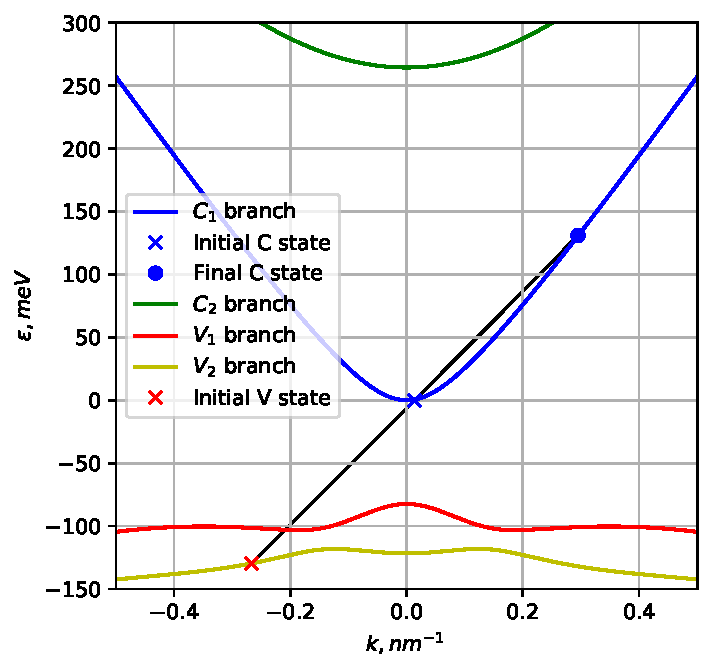
\includegraphics[width=\textwidth]{./images/add_pic.pdf}
            \end{center}
        \end{columns}
      \end{frame}

    \begin{frame}
        \frametitle{Пример: структура №170130}
        \begin{columns}
            \begin{column}{0.7\textwidth}
                \begin{overprint}
                    \onslide<1>
                    \begin{center}
                        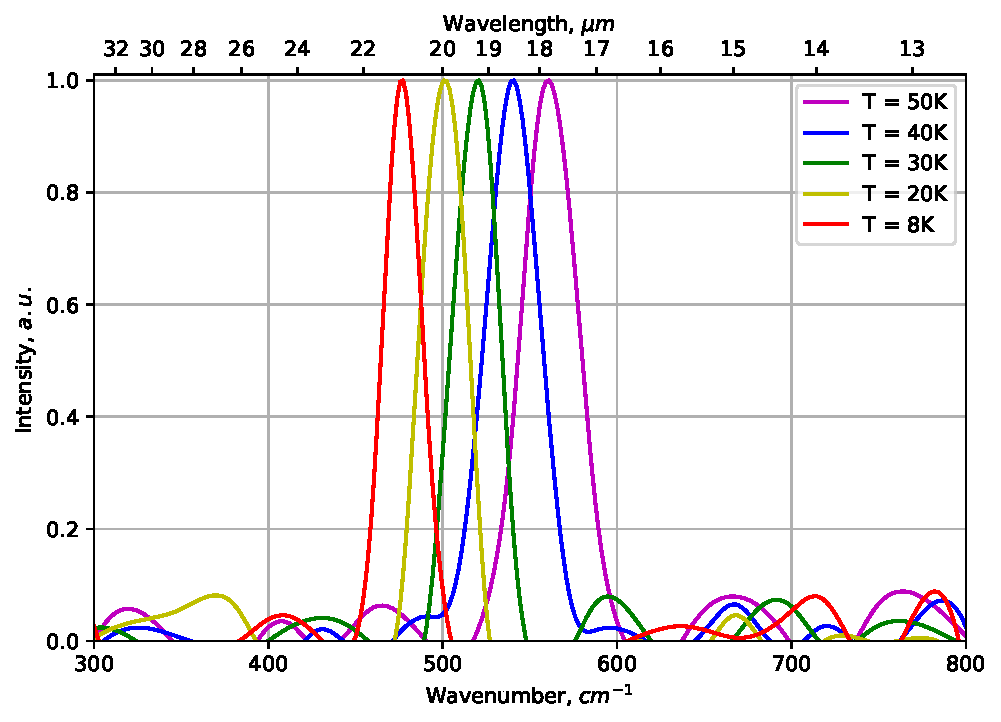
\includegraphics[width=\textwidth]{images/18um_spectre.pdf}
                    \end{center}
                    Спектр стимулированного излучения при разных температурах.

                    \onslide<2>
                    \begin{center}
                        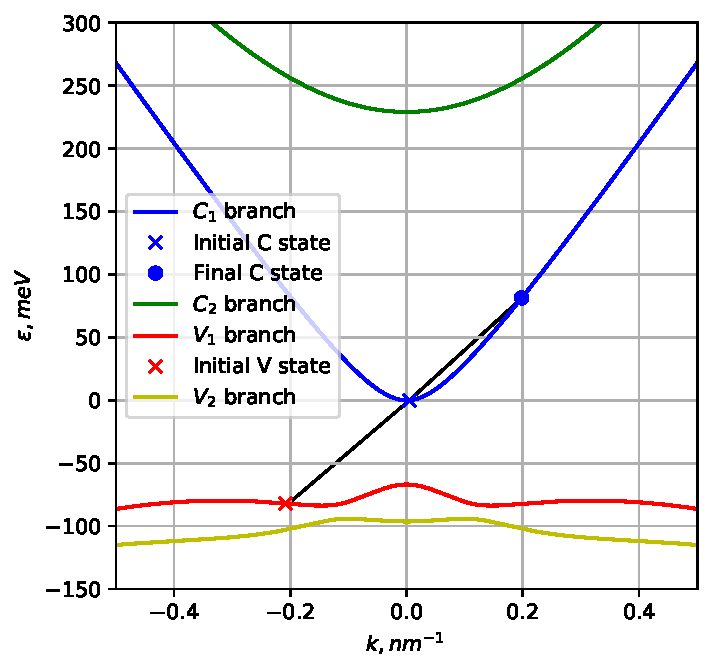
\includegraphics[width=1\textwidth]{images/18um_impure_40K.pdf}
                    \end{center}
                    Диаграма CCHC перехода, соответствующего $\varepsilon_\text{th}$.
                \end{overprint}
            \end{column}
            \hfill
            \begin{column}{0.3\textwidth}
                Свойства структуры:
                \begin{center}
                    \begin{tabular}{c | c c}
                        Prop.   & Val.  & [U.]\\
                        \hline
                        (hkl)       &  (013)    &\\
                        QW $\times$ &   10      &\\
                        $x_{QW}$    & 10   & \%\\
                        $d_{QW}$    & 8.7  & nm\\
                        $x_{bar}$  & 65   & \%\\
                        $\varepsilon_{g, 50K}$ & 70 & meV\\
                        $\varepsilon_{th, 50K}$  & 15 & meV\\
                        $T_{cr}$       & 50 & K
                    \end{tabular}
                \end{center}
            \end{column}
        \end{columns}
    \end{frame}

    \begin{frame}
        \frametitle{Повышение пороговой энергии: состав КЯ}
        \begin{columns}
            \begin{column}{0.7\textwidth}
                \begin{center}
                    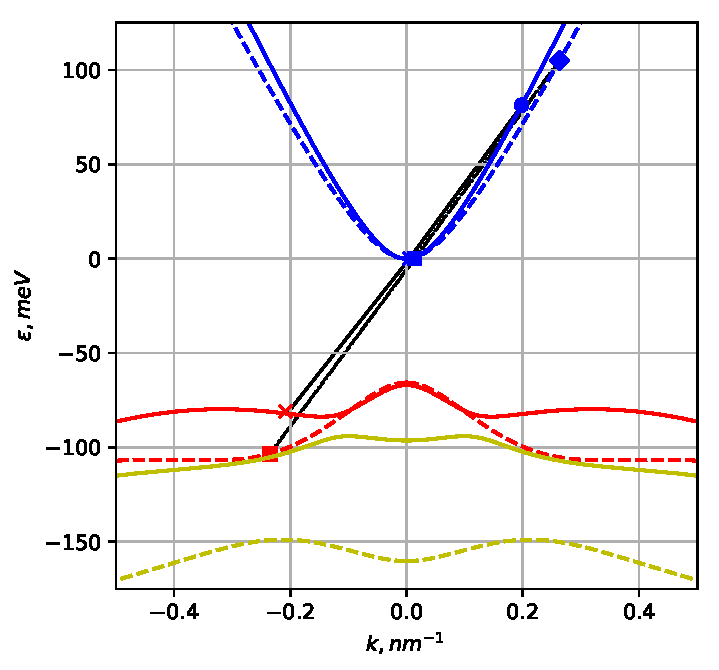
\includegraphics[width=1\textwidth]{images/18um_p_vs_i.pdf}
                \end{center}
                Сравнение пороговых оже-процессов структуры №170130
                и гипотетиеской с "чистыми" квантовыми ямами $x_{QW} = 0$.
            \end{column}
            \hfill
            \begin{column}{0.3\textwidth}
                \textit{Отсутствие боковых максимумов} в структуре с $x_{QW} = 0$
                приводит к повышению порога - следствие требования равенства 
                групповых скоростей.

                \vspace{3.5cm}
            \end{column}
        \end{columns}
    \end{frame}

    \begin{frame}
        \frametitle{Повышение пороговой энергии: состав барьеров}
        \begin{center}
            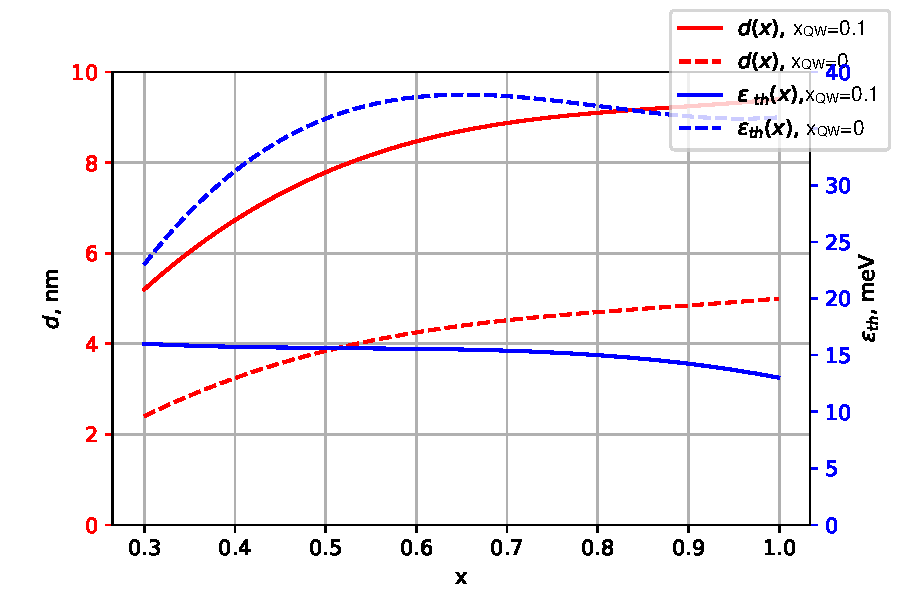
\includegraphics[width=1\textwidth]{images/de_vs_x_R.pdf}
        \end{center}
        Зависимость пороговой энергии оже-процессов и требуемой толщины КЯ
        при $\varepsilon_g \approx 70~meV$ и $T=40~K$.
    \end{frame}

    \begin{frame}
        \frametitle{Пример: структура №190225}
        \begin{columns}
            \begin{column}{0.7\textwidth}
                \begin{overprint}
                    \onslide<1>
                    \begin{center}
                        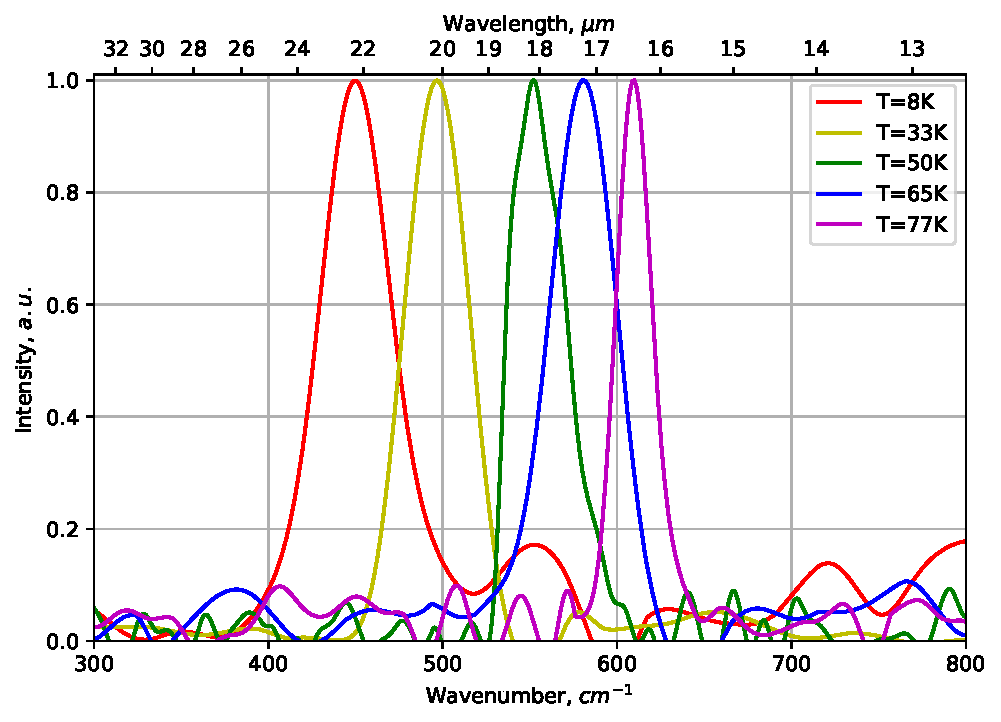
\includegraphics[width=\textwidth]{images/22um_spectre.pdf}
                    \end{center}
                    Спектр стимулированного излучения при разных температурах.

                    \onslide<2>
                    \begin{center}
                        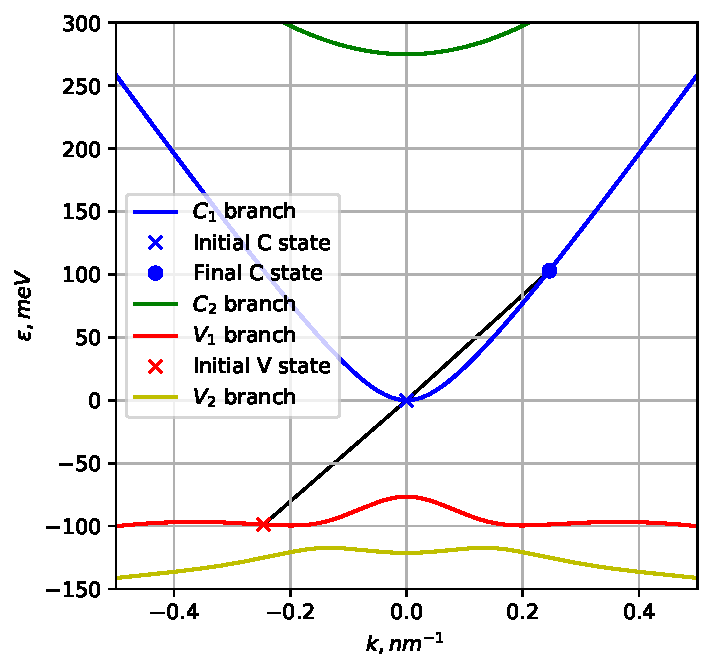
\includegraphics[width=1\textwidth]{images/22um_spec.pdf}
                    \end{center}
                    Диаграмма CCHC перехода, соответствующего $\varepsilon_\text{th}$ 
                    пороговой энергии.
                \end{overprint}
            \end{column}
            \hfill
            \begin{column}{0.3\textwidth}
                Свойства структуры:
                \begin{center}
                    \begin{tabular}{c | c c}
                        Prop.   & Val.  & [U.]\\
                        \hline
                        (hkl)       &  (013)    &\\
                        QW $\times$ &   11      &\\
                        $x_{QW}$    & 7.3   & \%\\
                        $d_{QW}$    & 6.8  & nm\\
                        $x_{bar}$  & 60   & \%\\
                        $x_{buf}$  & 65   & \%\\
                        $\varepsilon_{g, 77K}$ & 76 & meV\\
                        $\varepsilon_{th, 77K}$  & 23.5 & meV\\
                        $T_{cr}$       & 77 & K
                    \end{tabular}
                \end{center}
            \end{column}
        \end{columns}
    \end{frame}
    \begin{frame}
        \frametitle{Итоги:}
        \begin{itemize}
            \item Показана возможность расчёта пороговой энергии 
            оже-процессов для структур на основе HgCdTe.
            \item Продемонстрированна возможность повышения
            критической температуры путём изменения дисперсионных 
            соотношений.
            \item Получено стимулированное излучение на длине 
            волны $\lambda = 16~\mu m$ при температуре 
            кипения азота. 
        \end{itemize}

        \vspace{1.5cm}

        \begin{center}
            \large{Спасибо за внимание!}
        \end{center}
    \end{frame}
\end{document}